% COLORED HIGHLIGHT BEX -- \fcolorbox{bone}{lime}{Abib}
\chapter{Psalm 10}

\begin{figure}
  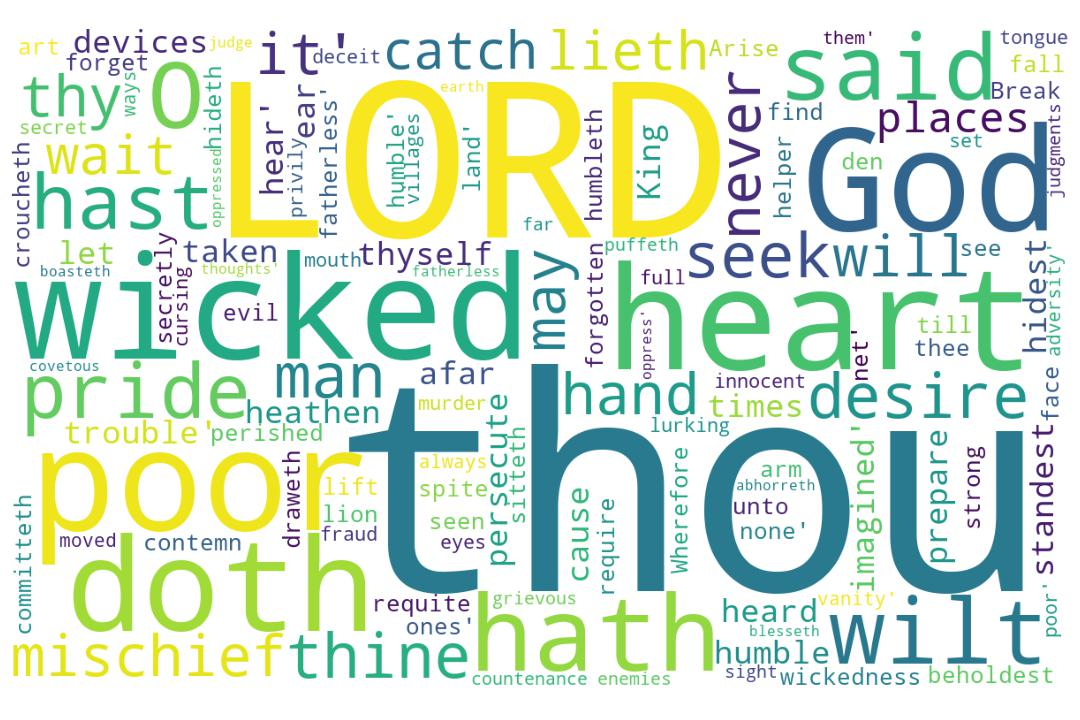
\includegraphics[width=\linewidth]{19OT-Psalms/Psalm10-WordCloud.jpg}
  \caption{Psalm 10 Word Cloud}
  \label{fig:Psalm 10 word Cloud}
\end{figure}


\marginpar{\scriptsize \centering \fcolorbox{bone}{lime}{\textbf{WHEN GOD SEEMS FAR AWAY}}\\ (Psalm 10:1-18)
\begin{compactenum}[I.][8]
    \item The \textbf{Evil Person} (Wicked) \index[scripture]{Psalms!Psa 010:02}\index[scripture]{Psalms!Psa 010:03}\index[scripture]{Psalms!Psa 010:04}\index[scripture]{Psalms!Psa 010:13}\index[scripture]{Psalms!Psa 010:15}(Psa 10:2, 3, 4, 13, 15) 
    \begin{compactenum}[A.]
	\item He persecutes \index[scripture]{Psalms!Psa 010:02}(Psa 10:2) 
    	\item He boasts \index[scripture]{Psalms!Psa 010:03}(Psa 10:3) 
   	\item He ignores God \index[scripture]{Psalms!Psa 010:04}(Psa 10:4) 
    	\item He curses \index[scripture]{Psalms!Psa 010:0}(Psa 10:7) 
    	\item He ambushes \index[scripture]{Psalms!Psa 010:08}(Psa 10:8) 
    	\item He Acts vindicated \index[scripture]{Psalms!Psa 010:11}(Psa 10:11) 
    \end{compactenum}
    \item An \textbf{Earnest Prayer} (Waiting) \index[scripture]{Psalms!Psa 010:12}(Psa 10:12) 
    \item An \textbf{Extended Preparation} (Withstand) \index[scripture]{Psalms!Psa 010:17}(Psa 10:17) 
    \item The \textbf{Enduring Promise} (Win) \index[scripture]{Psalms!Psa 010:18}(Psa 10:18) 
\end{compactenum}}


\marginpar{\scriptsize \centering \fcolorbox{bone}{yellow}{\textbf{10 MINUTES OF FAME}}\\ (Psalm 10:1-18)
\begin{compactenum}[I.][8]
    \item The \textbf{Strange Silence} \index[scripture]{Psalms!Psa 010:01}(Psa 10:1) 
    \item \textbf{Successful Sin} \index[scripture]{Psalms!Psa 010:02}(Psa 10:2) 
    \item \textbf{Scorning Statements Sin} \index[scripture]{Psalms!Psa 010:03}(Psa 10:3) 
    \item \textbf{Secret Seductions} \index[scripture]{Psalms!Psa 010:09}(Psa 10:9) 
    \item \textbf{Spiteful Speech} \index[scripture]{Psalms!Psa 010:13}(Psa 10:13) 
    \item The \textbf{Sweeping Slaughter} \index[scripture]{Psalms!Psa 010:15}(Psa 10:15) 
    \item A \textbf{Sovereign Supremacy} \index[scripture]{Psalms!Psa 010:16}(Psa 10:16) 
\end{compactenum}}

\footnote{\textcolor[cmyk]{0.99998,1,0,0}{\hyperlink{TOC}{Return to end of Table of Contents.}}}\footnote{\href{https://audiobible.com/bible/genesis_30.html}{\textcolor[cmyk]{0.99998,1,0,0}{Psalms Audio}}}\textcolor[cmyk]{0.99998,1,0,0}{Why\textcolor{jungle}{$_{2066}^{1}$} standest thou afar off, O LORD? \emph{why} hidest thou \emph{thyself} \underline{in} times of trouble?}\footnote{\textbf{Psalm 9:9} - The LORD also will be a refuge for the oppressed, a refuge in times of trouble.}
[2] \textcolor[cmyk]{0.99998,1,0,0}{The\textcolor{jungle}{$_{2081}^{16}$} \fcolorbox{bone}{lime}{wicked} \underline{in} \emph{his} pride doth persecute the poor: let them be taken \underline{in} the devices that they have imagined.}\footnote{\textbf{Job 41:34} - He beholdeth all high things: he is a king over all the children of pride.}
[3] \textcolor[cmyk]{0.99998,1,0,0}{For\textcolor{jungle}{$_{2101}^{36}$} the \fcolorbox{bone}{lime}{wicked} boasteth of his heart's desire, and blesseth the covetous, \emph{whom} the LORD abhorreth.}
[4] \textcolor[cmyk]{0.99998,1,0,0}{The\textcolor{jungle}{$_{2117}^{52}$} \fcolorbox{bone}{lime}{wicked}, through the pride of his countenance, will not seek \emph{after} \emph{God}: God \emph{is} not \underline{in} all his thoughts.}
[5] \textcolor[cmyk]{0.99998,1,0,0}{His\textcolor{jungle}{$_{2137}^{72}$} ways are always grievous; thy judgments \emph{are} far above out of his sight: \emph{as} \emph{for} all his enemies, he puffeth at them.}
[6] \textcolor[cmyk]{0.99998,1,0,0}{He\textcolor{jungle}{$_{2160}^{95}$} hath said \underline{in} his heart, I shall not be moved: for \emph{I} \emph{shall} never \emph{be} \underline{in} adversity.}
[7] \textcolor[cmyk]{0.99998,1,0,0}{His\textcolor{jungle}{$_{2178}^{113}$} mouth is full of cursing and deceit and fraud: under his tongue \emph{is} mischief and vanity.}
[8] \textcolor[cmyk]{0.99998,1,0,0}{He\textcolor{jungle}{$_{2195}^{130}$} sitteth \underline{in} the lurking places of the villages: \underline{in} the secret places doth he murder the innocent: his eyes are privily set against the poor.}
[9] \textcolor[cmyk]{0.99998,1,0,0}{He\textcolor{jungle}{$_{2221}^{156}$} lieth \underline{in} wait secretly as a lion \underline{in} his den: he lieth \underline{in} wait to catch the poor: he doth catch the poor, when he draweth him into his net.}\footnote{\textbf{1 Peter 5:8} - Be sober, be vigilant; because your adversary the devil, as a roaring lion, walketh about, seeking whom he may devour:}
[10] \textcolor[cmyk]{0.99998,1,0,0}{He\textcolor{jungle}{$_{2252}^{187}$} croucheth, \emph{and} humbleth himself, that the poor may fall by his strong ones.}
[11] \textcolor[cmyk]{0.99998,1,0,0}{He\textcolor{jungle}{$_{2266}^{201}$} hath said \underline{in} his heart, God hath forgotten: he hideth his face; he will never see \emph{it}.}
[12] \textcolor[cmyk]{0.99998,1,0,0}{Arise\textcolor{jungle}{$_{2284}^{219}$}, O LORD; O God, lift up thine hand: \fcolorbox{bone}{lime}{forget not the humble}.}
[13] \textcolor[cmyk]{0.99998,1,0,0}{Wherefore\textcolor{jungle}{$_{2297}^{232}$} doth the \fcolorbox{bone}{lime}{wicked} contemn God? he hath said \underline{in} his heart, Thou wilt not require \emph{it}.}
[14] \textcolor[cmyk]{0.99998,1,0,0}{Thou\textcolor{jungle}{$_{2314}^{249}$} hast seen \emph{it}; for thou beholdest mischief and spite, to requite \emph{it} with thy hand: the poor committeth himself unto thee; thou art the helper of the fatherless.}
[15] \textcolor[cmyk]{0.99998,1,0,0}{Break\textcolor{jungle}{$_{2343}^{278}$} thou the arm of the \fcolorbox{bone}{lime}{wicked} and the evil \emph{man}: seek out his wickedness \emph{till} thou find none.}\footnote{\textbf{Zechariah 11:17} -  Woe to the idol shepherd that leaveth the flock! the sword shall be upon his arm, and upon his right eye: his arm shall be clean dried up, and his right eye shall be utterly darkened.}
[16] \textcolor[cmyk]{0.99998,1,0,0}{The\textcolor{jungle}{$_{2362}^{297}$} LORD \emph{is} King for ever and ever: the heathen are perished out of his land.}
[17] \textcolor[cmyk]{0.99998,1,0,0}{LORD\textcolor{jungle}{$_{2378}^{313}$}, thou hast heard the desire of the humble: thou wilt \fcolorbox{bone}{lime}{prepare} their heart, thou wilt cause thine ear to hear:}
[18] \textcolor[cmyk]{0.99998,1,0,0}{To\textcolor{jungle}{$_{2399}^{334}$} judge the fatherless and the oppressed, that the man of the earth may \fcolorbox{bone}{lime}{no more oppress\textcolor{jungle}{$_{2415}^{350}$}}.}

